% Options for packages loaded elsewhere
\PassOptionsToPackage{unicode}{hyperref}
\PassOptionsToPackage{hyphens}{url}
\PassOptionsToPackage{dvipsnames,svgnames,x11names}{xcolor}
\documentclass[
  11pt,
]{article}
\usepackage{xcolor}
\usepackage[margin=1in]{geometry}
\usepackage{amsmath,amssymb}
\setcounter{secnumdepth}{5}
\usepackage{iftex}
\ifPDFTeX
  \usepackage[T1]{fontenc}
  \usepackage[utf8]{inputenc}
  \DeclareUnicodeCharacter{00D7}{\ensuremath{\times}}
  \DeclareUnicodeCharacter{00B2}{\ensuremath{^2}}
  \usepackage{textcomp} % provide euro and other symbols
\else % if luatex or xetex
  \usepackage{unicode-math} % this also loads fontspec
  \defaultfontfeatures{Scale=MatchLowercase}
  \defaultfontfeatures[\rmfamily]{Ligatures=TeX,Scale=1}
\fi
\usepackage{lmodern}
\ifPDFTeX\else
  % xetex/luatex font selection
\fi
% Use upquote if available, for straight quotes in verbatim environments
\IfFileExists{upquote.sty}{\usepackage{upquote}}{}
\IfFileExists{microtype.sty}{% use microtype if available
  \usepackage[]{microtype}
  \UseMicrotypeSet[protrusion]{basicmath} % disable protrusion for tt fonts
}{}
\makeatletter
\@ifundefined{KOMAClassName}{% if non-KOMA class
  \IfFileExists{parskip.sty}{%
    \usepackage{parskip}
  }{% else
    \setlength{\parindent}{0pt}
    \setlength{\parskip}{6pt plus 2pt minus 1pt}}
}{% if KOMA class
  \KOMAoptions{parskip=half}}
\makeatother
\usepackage{longtable,booktabs,array}
\newcounter{none} % for unnumbered tables
\usepackage{calc} % for calculating minipage widths
% Correct order of tables after \paragraph or \subparagraph
\usepackage{etoolbox}
\makeatletter
\patchcmd\longtable{\par}{\if@noskipsec\mbox{}\fi\par}{}{}
\makeatother
% Allow footnotes in longtable head/foot
\IfFileExists{footnotehyper.sty}{\usepackage{footnotehyper}}{\usepackage{footnote}}
\makesavenoteenv{longtable}
\usepackage{graphicx}
\makeatletter
\newsavebox\pandoc@box
\newcommand*\pandocbounded[1]{% scales image to fit in text height/width
  \sbox\pandoc@box{#1}%
  \Gscale@div\@tempa{\textheight}{\dimexpr\ht\pandoc@box+\dp\pandoc@box\relax}%
  \Gscale@div\@tempb{\linewidth}{\wd\pandoc@box}%
  \ifdim\@tempb\p@<\@tempa\p@\let\@tempa\@tempb\fi% select the smaller of both
  \ifdim\@tempa\p@<\p@\scalebox{\@tempa}{\usebox\pandoc@box}%
  \else\usebox{\pandoc@box}%
  \fi%
}
% Set default figure placement to htbp
\def\fps@figure{htbp}
\makeatother
\setlength{\emergencystretch}{3em} % prevent overfull lines
\providecommand{\tightlist}{%
  \setlength{\itemsep}{0pt}\setlength{\parskip}{0pt}}
\usepackage{bookmark}
\IfFileExists{xurl.sty}{\usepackage{xurl}}{} % add URL line breaks if available
\urlstyle{same}
\hypersetup{
  pdftitle={Milestone 2: Accelerating Neighbourhood Search in SPH},
  pdfauthor={Aditya Melinkeri, Ria Arora, Anirban Deshmukh, Prajakta Bandgar},
  colorlinks=true,
  linkcolor={blue},
  filecolor={Maroon},
  citecolor={Blue},
  urlcolor={blue},
  pdfcreator={LaTeX via pandoc}}

\title{Milestone 2: Accelerating Neighbourhood Search in SPH}
\author{Aditya Melinkeri \and Ria Arora \and Anirban Deshmukh \and Prajakta Bandgar}
\date{30 September 2026}

\usepackage{float}
\usepackage{fvextra}
\usepackage{etoolbox}
\usepackage[font=small,labelfont=bf]{caption}
\DefineVerbatimEnvironment{verbatim}{Verbatim}{breaklines=true,breakanywhere=true,fontsize=\small}
\AtBeginEnvironment{longtable}{\small}
\setcounter{tocdepth}{2}
\setcounter{secnumdepth}{2}
\setlength{\emergencystretch}{3em}

\microtypesetup{expansion=false}
\ifPDFTeX\pdfcompresslevel=1\pdfobjcompresslevel=0\fi
\captionsetup{justification=raggedright,singlelinecheck=false}

\begin{document}
\maketitle

{
\setcounter{tocdepth}{2}
\tableofcontents
\clearpage
}
This report follows the development of the CPU solver from the
sequential C++ baseline to OpenMP multithreading and then to spatial
hashing. The starting observation is that the baseline spends most of a
physics step finding neighbouring particles. The work therefore proceeds
in two stages: distribute particle calculations across CPU threads, then
reduce the number of candidate particles that those calculations
examine.

The discussion uses the existing source code, benchmark data, and
figures in the project. The earlier sequential measurements establish
where the project left off; the later comparison measurements evaluate
the sequential, OpenMP all-pairs, and OpenMP spatial-hash variants.
Results from separate measurement campaigns are identified where they
appear. All times are in milliseconds unless stated otherwise.

\section{Where we left off: sequential scaling and the
neighbourhood-search
bottleneck}\label{where-we-left-off-sequential-scaling-and-the-neighbourhood-search-bottleneck}

\subsection{The sequential C++
baseline}\label{the-sequential-c-baseline}

The sequential implementation provides the reference point for the
parallel work. It represents the fluid as particles and computes density
and force contributions by scanning every particle for each target
particle. A distance test determines whether a candidate falls within
the smoothing kernel's support. Candidates outside that support
contribute nothing, but the program still pays the cost of reading their
positions and computing their separation.

For a system containing N particles, one complete all-pairs pass
performs approximately N² candidate checks. The solver makes such a pass
for density and another for force evaluation. The exact work differs
between the two passes, but both have quadratic candidate-search
complexity. Doubling N therefore produces approximately four times as
many candidate checks per pass.

This baseline matters because the parallel implementation can retain the
same particle model and interaction calculations. Speedup can then be
measured against compiled sequential C++ rather than against the older
Python exploration.

\subsection{Scaling with particle
count}\label{scaling-with-particle-count}

The earlier sequential sweep used the hydrostatic scene and measured the
physics update without rendering. The initial particle spacing was
chosen to approach a requested particle count; the scene generator
rounded the lattice geometry, so the actual count can differ slightly
from the request.

\begin{figure}[H]
\centering
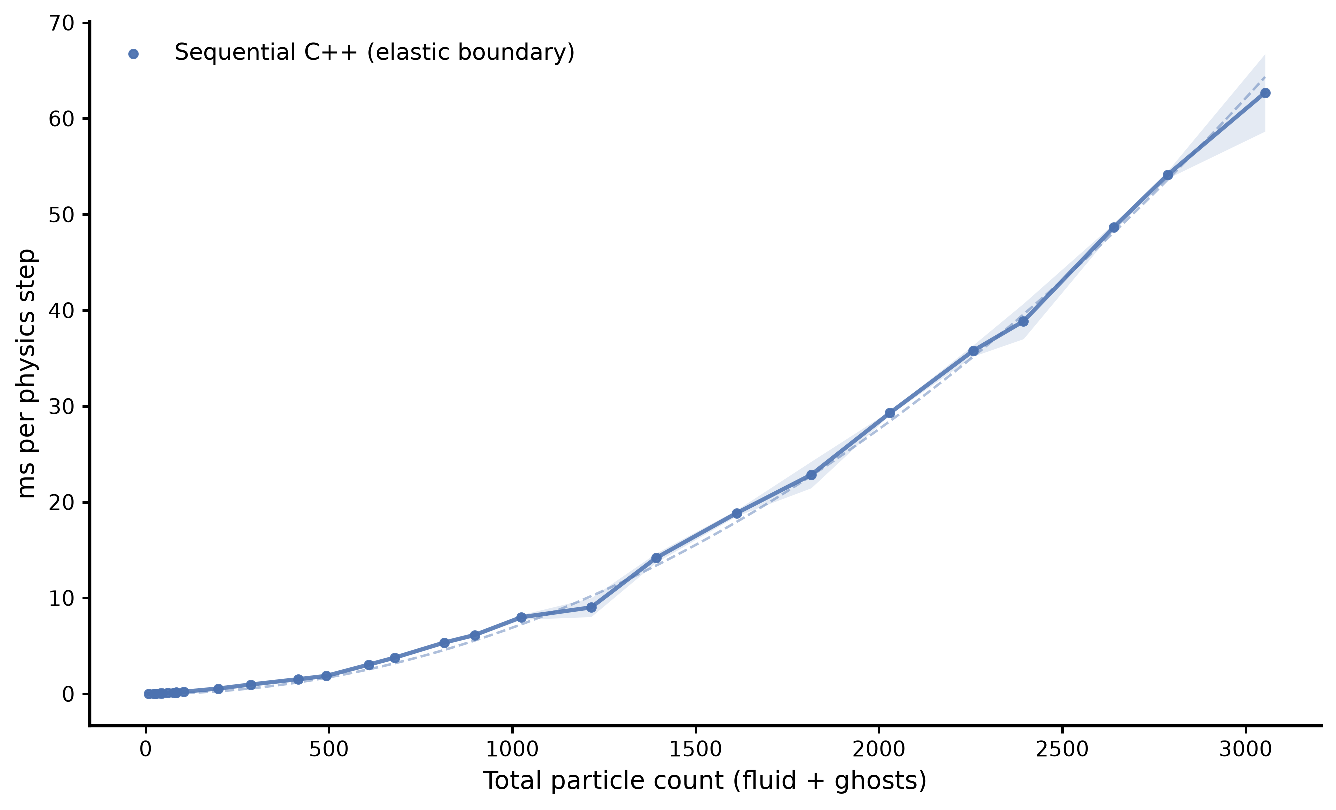
\includegraphics[page=1,width=\linewidth,height=0.48\textheight,keepaspectratio]{figures/report_figure_assets.pdf}
\caption{Earlier sequential scaling sweep. The increasing slope is
consistent with the quadratic growth expected from an all-pairs search.
The dashed curve is a quadratic fit. The saved figure's horizontal label
says ``fluid + ghosts,'' but the associated JSON records zero ghost
particles; the counts in this report are the actual fluid
counts.}\label{fig:1}
\end{figure}

{\def\LTcaptype{none} % do not increment counter
\begin{longtable}[]{@{}
  >{\raggedleft\arraybackslash}p{(\linewidth - 6\tabcolsep) * \real{0.2500}}
  >{\raggedleft\arraybackslash}p{(\linewidth - 6\tabcolsep) * \real{0.2500}}
  >{\raggedleft\arraybackslash}p{(\linewidth - 6\tabcolsep) * \real{0.2500}}
  >{\raggedleft\arraybackslash}p{(\linewidth - 6\tabcolsep) * \real{0.2500}}@{}}
\toprule\noalign{}
\begin{minipage}[b]{\linewidth}\raggedleft
Requested particles
\end{minipage} & \begin{minipage}[b]{\linewidth}\raggedleft
Actual fluid particles
\end{minipage} & \begin{minipage}[b]{\linewidth}\raggedleft
Mean time per step
\end{minipage} & \begin{minipage}[b]{\linewidth}\raggedleft
Standard deviation across 10-step windows
\end{minipage} \\
\midrule\noalign{}
\endhead
\bottomrule\noalign{}
\endlastfoot
500 & 493 & 1.873 & 0.113 \\
1,000 & 1,025 & 7.994 & 0.249 \\
2,000 & 2,030 & 29.299 & 0.198 \\
3,000 & 3,053 & 62.697 & 4.040 \\
\end{longtable}
}

The increase from 1,025 to 2,030 particles is close to a doubling of
problem size. Runtime increases by approximately 3.67×. Increasing the
count to 3,053 particles gives approximately 7.84× the runtime at 1,025
particles. Fixed costs, execution variability, and differences in the
particle state affect the exact ratios, but the overall curve clearly
becomes more expensive as the number of possible pairs grows.

The source for this sweep is the earlier sequential scaling dataset
(\path{sequential_c/data/scaling_results.json}). These values describe
that measurement campaign. Later sections use the sequential baseline
recorded alongside the parallel comparison campaign when calculating
cross-implementation speedups.

\subsection{Breaking down an average
timestep}\label{breaking-down-an-average-timestep}

A total runtime curve identifies poor scaling but does not identify
where the time is spent. The breakdown mode separates the physics update
into six measured categories:

{\def\LTcaptype{none} % do not increment counter
\begin{longtable}[]{@{}
  >{\raggedright\arraybackslash}p{(\linewidth - 4\tabcolsep) * \real{0.3333}}
  >{\raggedright\arraybackslash}p{(\linewidth - 4\tabcolsep) * \real{0.3333}}
  >{\raggedright\arraybackslash}p{(\linewidth - 4\tabcolsep) * \real{0.3333}}@{}}
\toprule\noalign{}
\begin{minipage}[b]{\linewidth}\raggedright
Stage
\end{minipage} & \begin{minipage}[b]{\linewidth}\raggedright
Operation
\end{minipage} & \begin{minipage}[b]{\linewidth}\raggedright
Purpose
\end{minipage} \\
\midrule\noalign{}
\endhead
\bottomrule\noalign{}
\endlastfoot
A & Density neighbourhood search & Find particles close enough to
contribute to density. \\
B & Density computation & Evaluate and accumulate kernel contributions
from the selected neighbours. \\
C & Force neighbourhood search & Find valid neighbours for pressure and
viscosity interactions. \\
D & Force computation & Evaluate the force contributions for the
selected neighbours. \\
E & Pressure computation & Convert density to pressure using the
equation of state. \\
F & Boundary handling & Apply the response at the domain walls. \\
\end{longtable}
}

\begin{figure}[H]
\centering
\includegraphics[page=2,width=\linewidth,height=0.48\textheight,keepaspectratio]{figures/report_figure_assets.pdf}
\caption{Earlier sequential breakdown at 2,030 fluid particles. The two
neighbourhood-search bars dominate the measured step.}\label{fig:2}
\end{figure}

{\def\LTcaptype{none} % do not increment counter
\begin{longtable}[]{@{}lr@{}}
\toprule\noalign{}
Stage & Mean time per step \\
\midrule\noalign{}
\endhead
\bottomrule\noalign{}
\endlastfoot
A --- Density neighbourhood search & 14.645 \\
B --- Density computation & 0.394 \\
C --- Force neighbourhood search & 16.953 \\
D --- Force computation & 1.715 \\
E --- Pressure computation & 0.015 \\
F --- Boundary handling & 0.003 \\
\textbf{Complete timed update in breakdown mode} & \textbf{33.773} \\
\end{longtable}
}

The two search stages take 31.598 ms together. Dividing this by the
complete timed update gives a \textbf{93.56\% search share}. The useful
density and force arithmetic is much smaller than the work required to
identify which particle pairs should participate in it.

The six bars do not exhaust every operation in the timed update.
Velocity and position updates, control flow, and timing overhead also
contribute to its total. In addition, breakdown mode explicitly
materializes temporary neighbour lists so it can time search separately
from arithmetic. It is a diagnostic execution path, and its total need
not equal the normal solver timing. Its stage proportions should be
interpreted within that path. The raw values are in the sequential
breakdown dataset (\path{sequential_c/data/breakdown_n2000.json}).

\subsection{The bottleneck becomes more pronounced at larger
N}\label{the-bottleneck-becomes-more-pronounced-at-larger-n}

The later comparison campaign also measured the sequential breakdown at
30,016 particles, matching the larger example used in the presentation.

\begin{figure}[H]
\centering
\includegraphics[page=3,width=\linewidth,height=0.48\textheight,keepaspectratio]{figures/report_figure_assets.pdf}
\caption{Sequential breakdown at 30,016 particles in the later campaign.
The density and force searches take approximately 1,096.64 and 1,162.81
ms respectively.}\label{fig:3}
\end{figure}

At this size, the searches occupy 2,259.45 ms of a 2,275.15 ms timed
update, or \textbf{99.31\%}. The evidence therefore gives a specific
optimization target. Improving pressure calculation alone would affect a
very small portion of runtime; accelerating neighbourhood search can
affect almost the whole step.

The next step is to identify which parts of the SPH update can run
concurrently and apply multithreading to the dominant loops.


\begin{figure}[H]
\centering
\includegraphics[page=4,width=1\linewidth,height=.48\textheight,keepaspectratio]{figures/report_figure_assets.pdf}
\caption{Sequential stage costs across the saved particle-count sweep. The two neighbourhood searches account for almost all of the growth, showing that the bottleneck persists across resolutions rather than being peculiar to the 30,016-particle example. Source: \texttt{\detokenize{parallel_c/data/breakdown_vs_n_sequential_t1.png}}.}\label{fig:seq-breakdown-sweep}
\end{figure}

\section{The SPH computation and opportunities for parallel
execution}\label{the-sph-computation-and-opportunities-for-parallel-execution}

\subsection{What a particle stores}\label{what-a-particle-stores}

Smoothed Particle Hydrodynamics is a particle-based representation of a
fluid. Each particle carries a position and velocity, while density,
pressure, and acceleration are calculated from the current state. A
smoothing kernel assigns a contribution according to the distance
between particles. Contributions vanish outside a finite support radius.

For clarity, this report uses H for the smoothing-length parameter used
in the code and R for the support radius. The implemented kernel has
support for distance less than 2H, so \textbf{R = 2H}. This distinction
is also used when choosing the spatial-grid cell size in Section 5.

The main state arrays contain positions, velocities, accelerations,
densities, and pressures. Most calculations read several of these arrays
but write only the result associated with one target particle. That
ownership pattern is the basis of the OpenMP implementation.


\begin{figure}[H]
\centering
\includegraphics[page=5,width=1\linewidth,height=.38\textheight,keepaspectratio]{figures/report_figure_assets.pdf}
\caption{Finite-support particle interactions, reproduced from slide 2 of the presentation. Only particles inside the support circle contribute to the target particle. The source illustration writes the support radius as $kh$; in this implementation the corresponding radius is $R=2H$.}\label{fig:sph-support}
\end{figure}

\subsection{Initialization and
density}\label{initialization-and-density}

Initialization establishes the particle positions, velocities, masses,
domain, and fluid parameters. For the benchmark scenes, particles begin
on a deterministic lattice. The validation driver derives H from the
initial spacing and configures the pressure stiffness from a
characteristic velocity. An initial force evaluation prepares the
acceleration needed by the integrator.

Density at particle i is calculated from the particles within the
support radius:

\[
\rho_i = \sum_{j\in\mathcal{N}(i)} m_j W(\lVert\mathbf{x}_i-\mathbf{x}_j\rVert,H).
\]

Here, W is the smoothing kernel and the neighbourhood contains the
particles whose contributions are nonzero. The density sum includes the
particle's own kernel contribution. The all-pairs implementation
discovers this neighbourhood by testing every candidate j.

Each density calculation reads positions and masses, then writes one
density value. Density for particle i does not depend on the newly
calculated density of another particle, so different target particles
can be assigned to different threads.

\subsection{Pressure and force
evaluation}\label{pressure-and-force-evaluation}

Once density is available, the implemented equation of state computes
pressure:

\[
p_i = K(\rho_i-\rho_0),
\]

where K is the pressure multiplier and rho-zero is the target density.
This is an elementwise operation. Every particle can calculate its
pressure independently after its density is ready.

Force evaluation then combines pressure interactions, viscosity, and
gravity. The pressure contribution uses the symmetric combination of
pressure divided by density squared for the two interacting particles.
The viscosity calculation depends on their relative positions and
velocities. The force loop skips self-interactions and zero-separation
pairs before evaluating the kernel gradient.

All target particles can evaluate their accelerations concurrently
provided the positions, velocities, densities, and pressures remain
stable during the force pass. Each target accumulates its own
acceleration. The program must finish density and pressure calculations
before allowing the force stage to read those arrays.

\subsection{Integration, boundaries, and the order of a
step}\label{integration-boundaries-and-the-order-of-a-step}

The benchmark driver uses a kick--drift--kick sequence. It advances
velocity by half a step using the previous acceleration, advances
position using that intermediate velocity, applies the wall response,
recalculates acceleration at the updated positions, and completes the
remaining half-velocity update.

\begin{verbatim}
Initialize positions and velocities
Calculate initial densities, pressures, and accelerations

Repeat for each timestep:
    Choose dt from the current velocity and acceleration limits
    Half kick: v[i] = v[i] + 0.5 * dt * a[i]
    Drift:     x[i] = x[i] + dt * v[i]
    Apply boundary response
    Calculate updated densities
    Calculate updated pressures
    Calculate updated accelerations
    Half kick: v[i] = v[i] + 0.5 * dt * a[i]
\end{verbatim}

The time-step selection uses both an acoustic limit and a force limit.
The code evaluates the maximum speed and acceleration, forms the two
limits, and chooses the smaller value. A parallel implementation could
calculate those maxima with reductions; the current benchmark driver
performs that scan serially and outside the timed update region.

The wall response is a per-particle clamp and velocity reflection with a
restitution factor. Although some existing labels call it an ``elastic''
boundary, the restitution factor need not equal one. These benchmark
runs use the wall-response path without adding ghost particles.


\begin{figure}[H]
\centering
\includegraphics[page=6,width=1\linewidth,height=.58\textheight,keepaspectratio]{figures/report_figure_assets.pdf}
\caption{The sequential SPH flow diagram from slide 3. This schematic introduces the density--pressure--force dependency and the recurrence between timesteps. The kick--drift--kick pseudocode above gives the more precise integration and boundary-update order used by the benchmark driver.}\label{fig:sequential-flow}
\end{figure}

\subsection{Parallelism and
synchronization}\label{parallelism-and-synchronization}

{\def\LTcaptype{none} % do not increment counter
\begin{longtable}[]{@{}
  >{\raggedright\arraybackslash}p{(\linewidth - 6\tabcolsep) * \real{0.2500}}
  >{\raggedright\arraybackslash}p{(\linewidth - 6\tabcolsep) * \real{0.2500}}
  >{\raggedright\arraybackslash}p{(\linewidth - 6\tabcolsep) * \real{0.2500}}
  >{\raggedright\arraybackslash}p{(\linewidth - 6\tabcolsep) * \real{0.2500}}@{}}
\toprule\noalign{}
\begin{minipage}[b]{\linewidth}\raggedright
Operation
\end{minipage} & \begin{minipage}[b]{\linewidth}\raggedright
Parallel work unit
\end{minipage} & \begin{minipage}[b]{\linewidth}\raggedright
Required input
\end{minipage} & \begin{minipage}[b]{\linewidth}\raggedright
Current parallel benchmark implementation
\end{minipage} \\
\midrule\noalign{}
\endhead
\bottomrule\noalign{}
\endlastfoot
Density & One target particle & Positions and kernel parameters & OpenMP
outer particle loop \\
Pressure & One density entry & Completed density values & OpenMP loops
inside vector arithmetic \\
Force & One target particle & Positions, velocities, densities,
pressures & OpenMP outer particle loop \\
Velocity updates & One particle & Acceleration and dt & OpenMP particle
loops \\
Position update & One particle & Intermediate velocity and dt & OpenMP
particle loop \\
Boundary response & One particle & Updated position and velocity &
Serial loop; independent per-particle work is available \\
Time-step limits & Reduction over particles & Speeds and accelerations &
Serial maximum scan in the driver \\
\end{longtable}
}

Synchronization follows the data dependencies. Updated positions must be
ready before neighbourhood evaluation. Densities and pressures must be
ready before force evaluation. New accelerations must be ready before
the second half kick. OpenMP worksharing barriers enforce the necessary
order in the current implementation.

Consecutive timesteps retain a sequential dependency because the next
step requires the previous step's particle state. The available
parallelism is therefore across particles within each stage.

\section{Multithreading with OpenMP}\label{multithreading-with-openmp}

\subsection{Distributing target
particles}\label{distributing-target-particles}

OpenMP provides shared-memory threading within a process. Threads can
read the same particle arrays while owning different output elements.
The all-pairs parallel variant preserves the search algorithm and
distributes the outer loop over target particles.

The sequential density structure is:

\begin{verbatim}
for i = 0 to N - 1:
    rho[i] = 0
    for j = 0 to N - 1:
        if distance(x[i], x[j]) < R:
            rho[i] += mass[j] * W(x[i], x[j])
\end{verbatim}

The OpenMP version changes how the outer iterations are executed:

\begin{verbatim}
// Illustrative pseudocode; each iteration owns rho[i].
#pragma omp parallel for schedule(static)
for (int i = 0; i < N; ++i) {
    double density = 0.0;
    for (int j = 0; j < N; ++j) {
        if (distance(x[i], x[j]) < R)
            density += mass[j] * W(x[i], x[j]);
    }
    rho[i] = density;
}
// The loop completes before the next dependent stage begins.
\end{verbatim}

Each iteration accumulates the density for one target. Two threads do
not update the same density entry, so the algorithm does not require an
atomic operation for every interaction. The local accumulator in this
pseudocode makes that ownership explicit; the implementation also
achieves ownership by assigning each outer-loop index to one thread.

Static scheduling suits the all-pairs pass because every target
initially scans the same number of candidates. The amount of force
arithmetic can still vary with the number of accepted neighbours, but
candidate scanning dominates this version.


\begin{figure}[H]
\centering
\includegraphics[page=7,width=1\linewidth,height=.62\textheight,keepaspectratio]{figures/report_figure_assets.pdf}
\caption{Particle-level work sharing and stage barriers, reproduced from slide 7. The illustrated particle tasks are distributed over a fixed pool of OpenMP threads; the implementation does not create a separate operating-system thread for every particle. Pressure is shown as one stage here, and its elementwise vector operations are also threaded in the code.}\label{fig:parallel-flow}
\end{figure}

\subsection{Parallel pressure and force
calculations}\label{parallel-pressure-and-force-calculations}

Pressure calculation is expressed in the source as vector subtraction
followed by vector multiplication. The parallel vector implementation
contains OpenMP loops for those operations. It therefore contributes
parallel-region and intermediate-array costs even though the pressure
expression itself is compact.

\begin{verbatim}
After every density is available:
    parallel for i = 0 to N - 1:
        pressure[i] = K * (density[i] - rest_density)

After every pressure is available:
    parallel for each fluid particle i:
        a_local = gravity
        for j = 0 to N - 1:
            if i != j and separation is valid and distance(i, j) < R:
                a_local += pressure_contribution(i, j)
                a_local += viscosity_contribution(i, j)
        acceleration[i] = a_local
\end{verbatim}

The pressure pseudocode shows the logical elementwise operation; the
current vector expression implements it as separate arithmetic passes.
The force pseudocode retains the target-owned accumulation used by the
solver.

A pair may be visited once while evaluating i and again while evaluating
j. Computing each pair only once would require coordinating updates to
two particles, for example through atomics, private buffers, or another
accumulation scheme. The current design accepts the repeated pair visit
to keep writes independent and the threaded loop straightforward.

\subsection{Parallel integration with ordered
stages}\label{parallel-integration-with-ordered-stages}

The same ownership principle applies to the integration loops:

\begin{verbatim}
dt = choose_timestep(current_state)

parallel for each fluid particle i:
    velocity[i] += 0.5 * dt * acceleration[i]

parallel for each fluid particle i:
    position[i] += dt * velocity[i]

apply_boundary_response()              // serial in the current driver
update_density_pressure_and_forces()   // ordered stages described above

parallel for each fluid particle i:
    velocity[i] += 0.5 * dt * acceleration[i]
\end{verbatim}

Each \texttt{parallel\ for} completes before the next dependent
operation. This prevents one stage from observing a mixture of old and
updated particle data. The pseudocode follows the benchmark driver's
integration path, which performs these steps explicitly.

\subsection{Expected performance and remaining
work}\label{expected-performance-and-remaining-work}

If the expensive work divided perfectly over P threads, its elapsed time
would approach the sequential time divided by P. Actual performance also
includes serial work, barriers, parallel-region management, cache
effects, and memory traffic. For small N, those costs can be comparable
to the useful work assigned to each thread.

Multithreading still leaves approximately two all-pairs candidate passes
per update. At fixed P, the dominant work remains proportional to N².
The implementation can lower the runtime curve while retaining its
quadratic shape. The next section checks both the speedup and the
remaining stage distribution.

The relevant implementation is the OpenMP all-pairs solver
(\path{parallel_c/prehash/physics_prehash.cpp}), with integration in the
parallel benchmark driver (\path{parallel_c/validate_main.cpp}) and
threaded pressure operations in the vector implementation
(\path{parallel_c/backend/linalg.cpp}).

\section{Multithreading results: scaling with threads and the remaining
bottleneck}\label{multithreading-results-scaling-with-threads-and-the-remaining-bottleneck}

\subsection{How the comparison is
measured}\label{how-the-comparison-is-measured}

The later comparison uses three variants: sequential C++, OpenMP
all-pairs (labelled \texttt{prehash} in the data), and OpenMP with the
spatial grid (labelled \texttt{hash}). The benchmark harness generates a
hydrostatic lattice, runs a headless executable, and records the mean of
10-step window averages. Standard deviation describes the variation
between those windows.

The timer surrounds the velocity updates, position update, boundary
handling, and density/pressure/force evaluation. Scene setup, rendering,
snapshot output, and time-step selection are outside this interval. The
metric therefore describes the timed physics-update region rather than
the entire process wall time.

\begin{figure}[H]
\centering
\includegraphics[page=8,width=\linewidth,height=0.48\textheight,keepaspectratio]{figures/report_figure_assets.pdf}
\caption{Sequential and OpenMP all-pairs scaling for one through 32
threads. Additional threads reduce runtime, while the curves retain the
strong upward curvature associated with all-pairs work.}\label{fig:4}
\end{figure}

The sequential and one-thread OpenMP curves are close over much of the
range. This supports using the one-thread OpenMP run as a denominator
for thread scaling and the separately compiled sequential run as a
reference for the full implementation comparison.

\subsection{Strong scaling at approximately 10,000
particles}\label{strong-scaling-at-approximately-10000-particles}

Holding the particle count fixed while increasing the thread count
measures strong scaling. Define speedup and thread efficiency as:

\[
S(P)=\frac{T_{\mathrm{OpenMP},1}}{T_{\mathrm{OpenMP},P}},
\qquad E(P)=\frac{S(P)}{P}.
\]

At an actual count of 9,933 particles, the saved measurements are:

{\def\LTcaptype{none} % do not increment counter
\begin{longtable}[]{@{}
  >{\raggedleft\arraybackslash}p{(\linewidth - 6\tabcolsep) * \real{0.2500}}
  >{\raggedleft\arraybackslash}p{(\linewidth - 6\tabcolsep) * \real{0.2500}}
  >{\raggedleft\arraybackslash}p{(\linewidth - 6\tabcolsep) * \real{0.2500}}
  >{\raggedleft\arraybackslash}p{(\linewidth - 6\tabcolsep) * \real{0.2500}}@{}}
\toprule\noalign{}
\begin{minipage}[b]{\linewidth}\raggedleft
Threads
\end{minipage} & \begin{minipage}[b]{\linewidth}\raggedleft
OpenMP all-pairs time per step
\end{minipage} & \begin{minipage}[b]{\linewidth}\raggedleft
Speedup against one-thread OpenMP
\end{minipage} & \begin{minipage}[b]{\linewidth}\raggedleft
Thread efficiency
\end{minipage} \\
\midrule\noalign{}
\endhead
\bottomrule\noalign{}
\endlastfoot
1 & 327.232 & 1.00× & 100.0\% \\
2 & 172.769 & 1.89× & 94.7\% \\
4 & 92.969 & 3.52× & 88.0\% \\
8 & 50.911 & 6.43× & 80.3\% \\
16 & 28.047 & 11.67× & 72.9\% \\
24 & 26.904 & 12.16× & 50.7\% \\
32 & 27.424 & 11.93× & 37.3\% \\
\end{longtable}
}

The separate sequential executable takes 327.258 ms at this particle
count, giving approximately \textbf{12.16× speedup} for 24-thread OpenMP
against that baseline as well. The largest reductions occur before 16
threads. Moving from 16 to 24 threads gives a smaller improvement, and
32 threads are slightly slower in this particular measurement.

These results indicate diminishing returns at this workload size. They
do not identify a single hardware cause: synchronization, available
execution resources, memory behavior, and runtime variation can all
contribute. At larger N, 32 threads can still outperform 24 because more
work is available per thread.

\subsection{Thread scaling across the full particle-count sweep}\label{why-small-particle-counts-behave-differently}

The fuller saved sweep contains 49 particle counts for each of seven OpenMP thread settings, from 1 to 32 threads. Figure~\ref{fig:5} replaces the earlier five-count speedup plot with all 343 all-pairs measurements from the common benchmark dataset. For every particle count, the speedup is calculated as the one-thread time divided by the time at the chosen thread count. No new solver runs are used.

\begin{figure}[H]
\centering
\includegraphics[page=9,width=1\linewidth,height=.72\textheight,keepaspectratio]{figures/report_figure_assets.pdf}
\caption{OpenMP all-pairs thread scaling from the complete saved sweep. Panel (a) shows all 49 particle counts for each thread setting; panel (b) holds the particle count fixed and varies the number of threads. Speedups use mean per-step times in \texttt{\detokenize{parallel_c/data/scaling_results.json}}. Lines join measured values; the dashed reference in panel (b) is ideal linear speedup.}\label{fig:5}
\end{figure}

The two views answer complementary questions. The first shows how much useful work is available to amortize thread-management and synchronization costs as the particle count increases. The second shows diminishing returns when more threads are assigned to a fixed problem. Thread count alone cannot guarantee a speedup: the workload size, serial stages, memory behavior, and measurement variation all influence the result. The 9,933-particle values agree with the detailed table in Section 4.2 because both use the same dataset.

\subsection{Breakdown after
multithreading}\label{breakdown-after-multithreading}

\begin{figure}[H]
\centering
\includegraphics[page=10,width=\linewidth,height=0.48\textheight,keepaspectratio]{figures/report_figure_assets.pdf}
\caption{OpenMP all-pairs breakdown at 30,016 particles with 24 threads.
Searches are faster than in Figure~\ref{fig:3}, but still dominate the
step.}\label{fig:6}
\end{figure}

{\def\LTcaptype{none} % do not increment counter
\begin{longtable}[]{@{}
  >{\raggedright\arraybackslash}p{(\linewidth - 4\tabcolsep) * \real{0.2727}}
  >{\raggedleft\arraybackslash}p{(\linewidth - 4\tabcolsep) * \real{0.3636}}
  >{\raggedleft\arraybackslash}p{(\linewidth - 4\tabcolsep) * \real{0.3636}}@{}}
\toprule\noalign{}
\begin{minipage}[b]{\linewidth}\raggedright
Stage
\end{minipage} & \begin{minipage}[b]{\linewidth}\raggedleft
Sequential breakdown
\end{minipage} & \begin{minipage}[b]{\linewidth}\raggedleft
OpenMP all-pairs, 24 threads
\end{minipage} \\
\midrule\noalign{}
\endhead
\bottomrule\noalign{}
\endlastfoot
Density neighbourhood search & 1,096.639 & 81.072 \\
Density computation & 3.363 & 0.962 \\
Force neighbourhood search & 1,162.807 & 93.502 \\
Force computation & 12.076 & 1.291 \\
Pressure computation & 0.066 & 0.676 \\
Boundary handling & 0.018 & 0.061 \\
\textbf{Complete timed update in breakdown mode} & \textbf{2,275.148} &
\textbf{178.329} \\
\end{longtable}
}

Multithreading reduces this breakdown-mode total by approximately
12.76×. The two search stages fall from 2,259.45 ms to 174.57 ms, but
they still account for \textbf{97.89\%} of the OpenMP step. Their
absolute cost is lower; their dominance remains.

The table also shows that individual cheap stages do not necessarily
improve with threading. For example, pressure evaluation takes longer in
this run. Its vector operations create short parallel passes, for which
parallel overhead can exceed the benefit. A small-stage timing should be
interpreted with its measurement variability, but the broader result is
clear: nearly all remaining time is still spent in search.

\begin{figure}[H]
\centering
\includegraphics[page=11,width=\linewidth,height=0.48\textheight,keepaspectratio]{figures/report_figure_assets.pdf}
\caption{Stage costs across particle counts for the 24-thread all-pairs
variant. The two search curves dominate and continue to grow
sharply.}\label{fig:7}
\end{figure}

The all-pairs search therefore remains the limiting algorithm.
Additional CPU threads divide its work across more workers; the next
optimization must reduce the work that each target particle needs to
perform.

\section{Spatial hashing, neighbourhood queries, and CSR-like
storage}\label{spatial-hashing-neighbourhood-queries-and-csr-like-storage}

\subsection{Using the finite interaction
radius}\label{using-the-finite-interaction-radius}

The smoothing kernel already tells us that distant particles cannot
contribute. Spatial hashing organizes particles by position so those
distant candidates can be skipped before calculating their pairwise
separation.

The implementation uses a uniform grid over the bounded domain. Each
cell is assigned a flattened integer ID, and each particle is placed in
the cell containing its position. The repository refers to this as a
spatial hash. More specifically, it is a directly indexed grid of
particle buckets: the finite grid provides a unique cell index without a
general-purpose hash table or hash-collision resolution.

The cell side is chosen as R = 2H, matching the kernel support. In two
dimensions, any particle less than R away from a target must lie in the
same cell or one of the eight cells touching it. A query therefore
examines a 3×3 region:

\noindent\begin{minipage}{\linewidth}
\begin{verbatim}
             Candidate cells around the target cell

                +---------+---------+---------+
                | NW      | N       | NE      |
                +---------+---------+---------+
                | W       | target  | E       |
                +---------+---------+---------+
                | SW      | S       | SE      |
                +---------+---------+---------+

              Cell side = R = 2H; query 9 cells in 2D.
\end{verbatim}
\end{minipage}\par

The cell query provides a conservative candidate set. The program still
applies the exact distance test to each candidate because a square cell
region includes points outside the circular kernel support. In three
dimensions the same idea uses 27 nearby cells, but the present solver
and measurements are two-dimensional.


\begin{figure}[H]
\centering
\includegraphics[page=12,width=1\linewidth,height=.45\textheight,keepaspectratio]{figures/report_figure_assets.pdf}
\caption{Spatial-hashing illustration from slide 9. The green particle is the query target; blue particles pass the radius test; grey particles lie in candidate cells but still require a distance check; red particles lie outside the searched cell neighbourhood. The source diagram labels its interaction radius $h$; this report uses $R=2H$ for that radius and the cell side. The queried region comprises the target cell and its eight adjacent cells, nine cells in total.}\label{fig:spatial-hash-grid}
\end{figure}

\subsection{Mapping a position to a
cell}\label{mapping-a-position-to-a-cell}

For domain origin (xmin, ymin), cell side s = R, and grid width Cx, the
cell coordinates and flattened index are:

\[
c_x=\left\lfloor\frac{x-x_{\min}}{s}\right\rfloor,\qquad
c_y=\left\lfloor\frac{y-y_{\min}}{s}\right\rfloor,\qquad
c=c_x+c_y C_x.
\]

The origin subtraction places the grid in the correct world-coordinate
frame. The driver sizes the grid from the scene domain and includes room
for the upper edge. The implementation clamps cell coordinates to valid
ranges when assigning particles, preventing a particle exactly on a
boundary from generating an invalid array index.

Cell IDs are recalculated after particles move. A previously built grid
could otherwise contain outdated membership and omit newly nearby
particles. The current solver rebuilds the grid during each force-update
call, then uses that grid for both density and force queries at the same
particle positions.

\subsection{Why use a CSR-like
representation?}\label{why-use-a-csr-like-representation}

A cell needs to store a variable number of particle IDs. Allocating a
maximum-length particle array for every cell would waste memory, and
maintaining a separate dynamically allocated container per cell would
introduce additional allocation and traversal overhead.

The implemented representation places all particle IDs in one contiguous
array. Another array stores the beginning of each cell's range. This
resembles compressed sparse row storage: a cell acts like a row,
\texttt{cell\_start} acts like row offsets, and \texttt{cell\_particles}
holds the entries belonging to those rows.

{\def\LTcaptype{none} % do not increment counter
\begin{longtable}[]{@{}
  >{\raggedright\arraybackslash}p{(\linewidth - 4\tabcolsep) * \real{0.3000}}
  >{\raggedleft\arraybackslash}p{(\linewidth - 4\tabcolsep) * \real{0.4000}}
  >{\raggedright\arraybackslash}p{(\linewidth - 4\tabcolsep) * \real{0.3000}}@{}}
\toprule\noalign{}
\begin{minipage}[b]{\linewidth}\raggedright
Array
\end{minipage} & \begin{minipage}[b]{\linewidth}\raggedleft
Length
\end{minipage} & \begin{minipage}[b]{\linewidth}\raggedright
Meaning
\end{minipage} \\
\midrule\noalign{}
\endhead
\bottomrule\noalign{}
\endlastfoot
\texttt{cell\_id} & N & Cell containing each particle. \\
\texttt{cell\_count} & C & Number of particles assigned to each grid
cell. \\
\texttt{cell\_start} & C + 1 & Start offsets, including a sentinel at
the end. \\
\texttt{cell\_particles} & N & Particle IDs grouped by cell. \\
Temporary \texttt{cursor} & C & Next free slot in each cell's range
during construction. \\
\end{longtable}
}

If cell c starts at offset \texttt{cell\_start{[}c{]}} and the next cell
starts at \texttt{cell\_start{[}c+1{]}}, all its members are stored in
the half-open range between those offsets. An empty cell has equal start
and end offsets. The final sentinel equals N.

\subsection{Worked example of
construction}\label{worked-example-of-construction}

Consider seven particles distributed across four cells:

\begin{verbatim}
Particle ID:       0  1  2  3  4  5  6
Assigned cell:     2  0  2  1  0  3  2

cell_count:       [2, 1, 3, 1]
cell_start:       [0, 2, 3, 6, 7]
cell_particles:   [1, 4, 3, 0, 2, 6, 5]
                   ----  -  -------  -
                    c0  c1     c2   c3
\end{verbatim}

Cell 2 contains three particles. Its range starts at offset 3 and ends
before offset 6, so its particle IDs are \texttt{{[}0,\ 2,\ 6{]}}.
Retrieving that cell requires reading two offsets and traversing three
entries. It does not require searching all seven particles.

The prefix sum converts counts into non-overlapping output ranges.
Scattering each particle ID into its cell's range then completes the
representation. This groups indices by cell; it does not physically
reorder every particle state array or allocate a full list of
particle-to-particle neighbours.

\subsection{Construction pseudocode and parallel
work}\label{construction-pseudocode-and-parallel-work}

\begin{verbatim}
function build_grid(position, N, C):
    parallel for i = 0 to N - 1:
        cx = floor((position[i].x - xmin) / R)
        cy = floor((position[i].y - ymin) / R)
        clamp cx and cy to valid grid coordinates
        cell_id[i] = cx + cy * grid_width

    fill cell_count with zero

    for i = 0 to N - 1:
        cell_count[cell_id[i]] += 1

    cell_start[0] = 0
    for c = 0 to C - 1:
        cell_start[c + 1] = cell_start[c] + cell_count[c]

    cursor = copy of cell_start[0 : C]
    for i = 0 to N - 1:
        c = cell_id[i]
        cell_particles[cursor[c]] = i
        cursor[c] += 1
\end{verbatim}

The current implementation parallelizes particle-to-cell assignment.
Counting, prefix summation, and scattering are serial. This avoids races
in increments to shared cell counters and cursors. Making those
construction stages parallel would require an explicit coordination
strategy, such as per-thread counts or atomic updates; the current
results already include their serial cost.

\subsection{Querying the grid for density and
force}\label{querying-the-grid-for-density-and-force}

\begin{verbatim}
function candidates_for(i):
    for each valid cell c in the 3x3 region around particle i:
        for k = cell_start[c] to cell_start[c + 1] - 1:
            yield cell_particles[k]

build_grid(updated_positions)

parallel for each particle i:
    density[i] = 0
    for j in candidates_for(i):
        if distance(i, j) < R:
            density[i] += mass[j] * W(i, j)

calculate pressures from completed densities

parallel for each fluid particle i:
    acceleration[i] = gravity
    for j in candidates_for(i):
        if i != j and separation is valid and distance(i, j) < R:
            acceleration[i] += pressure_contribution(i, j)
            acceleration[i] += viscosity_contribution(i, j)
\end{verbatim}

This pseudocode expresses the geometric query and uses coordinate bounds
to identify valid neighbouring cells. The current source uses flattened
cell-ID offsets and checks their global index range. At a row edge, that
shortcut can enumerate extra wrapped cells; the exact distance filter
remains necessary. The intended candidate region is the 3×3
neighbourhood shown above.

The density and force formulas and target-owned threading structure
remain conceptually the same as before. The inner loop now visits
particles in nearby buckets instead of scanning the full particle array.
A completed grid is read-only while those queries execute, so multiple
threads can traverse its ranges concurrently.

\subsection{Time and memory
complexity}\label{time-and-memory-complexity}

Let C be the number of grid cells and k-bar the average number of
candidates visited per target particle. Building the grid requires O(N +
C) work: assign N particles, clear and prefix-sum C cells, and scatter N
indices. Querying all particles requires O(N × k-bar) candidate work. A
useful model for the complete search is therefore:

\[
T_{\mathrm{search}}=O(N+C+N\bar{k}).
\]

When cell occupancy remains bounded and C grows no faster than N, the
expected search cost is approximately O(N). This condition fits the
benchmark's resolution scaling: the driver sets H proportional to
particle spacing, so refining the initial lattice also reduces the
support radius and cell size. The typical initial number of particles in
a support region stays approximately constant.

This is not an unconditional worst-case guarantee. If many particles
accumulate in a few cells, a query must visit more candidates.
Increasing N in a fixed domain while keeping H fixed would also change
the occupancy assumption. The near-linear claim is tied to the tested
scene family and its smoothing-length choice.

The grid arrays require N entries for \texttt{cell\_id}, N for
\texttt{cell\_particles}, C for \texttt{cell\_count}, C + 1 for
\texttt{cell\_start}, and C temporary cursor entries. The construction
peak is therefore approximately \textbf{2N + 3C + 1 integer entries},
excluding the physical state arrays and allocation overhead. Memory is
O(N + C), becoming \textbf{O(N)} when C = O(N), as in this benchmark
setup. The main solver avoids storing an N-by-N neighbour matrix. The
diagnostic breakdown path does additionally materialize neighbour lists
to time search and arithmetic separately; that extra storage is distinct
from the grid representation itself.

\section{Spatial-hashing results: scaling, breakdown, and evidence of
improvement}\label{spatial-hashing-results-scaling-breakdown-and-evidence-of-improvement}

\subsection{Scaling across particle
counts}\label{scaling-across-particle-counts}

\begin{figure}[H]
\centering
\includegraphics[page=13,width=\linewidth,height=0.48\textheight,keepaspectratio]{figures/report_figure_assets.pdf}
\caption{OpenMP spatial-hash scaling over the tested particle-count
range. The dashed fits in this plot assume linear scaling; the
supporting evidence is the measured trend together with the
bounded-neighbour argument, rather than the fitted line
alone.}\label{fig:8}
\end{figure}

The one-thread spatial-grid implementation takes approximately 7.805 ms
at 9,933 particles, 25.632 ms at 30,016, and 76.469 ms at 99,960.
Increasing the count by roughly ten times from the first to the last
point increases runtime by approximately 9.80×. This is consistent with
near-linear growth across those endpoints and is substantially different
from the all-pairs scaling.

The curves contain local spikes and variability, so the measured
behavior is not a perfectly straight line. The data does not establish
the cause of each spike. The broad trend nevertheless shows that the
grid makes much larger particle counts practical within the measured CPU
update cost.

\subsection{Thread scaling after spatial
hashing}\label{thread-scaling-after-spatial-hashing}

At 99,960 particles, the spatial-hash variant has the following thread
scaling:

{\def\LTcaptype{none} % do not increment counter
\begin{longtable}[]{@{}rrr@{}}
\toprule\noalign{}
Threads & Time per step & Speedup against one-thread spatial hash \\
\midrule\noalign{}
\endhead
\bottomrule\noalign{}
\endlastfoot
1 & 76.469 & 1.00× \\
2 & 39.932 & 1.91× \\
4 & 22.702 & 3.37× \\
8 & 13.660 & 5.60× \\
16 & 10.954 & 6.98× \\
24 & 10.737 & 7.12× \\
32 & 10.171 & 7.52× \\
\end{longtable}
}

The grid and multithreading work together: the grid reduces candidate
work and OpenMP distributes the remaining particle calculations.
However, the reduced work per target makes other costs more significant.
Serial grid construction, barriers, pressure passes, boundary work, and
memory accesses now represent a larger fraction of runtime. The current
measurements show much smaller gains above 16 threads than below it.

At approximately 10,000 particles, the saved spatial-hash measurements
are fastest at eight threads among the tested choices: approximately
1.660 ms, compared with 1.844 ms at 24 threads. The best thread count
therefore depends on problem size and should not be assumed to be the
largest available count.


\begin{figure}[H]
\centering
\includegraphics[page=14,width=1\linewidth,height=.72\textheight,keepaspectratio]{figures/report_figure_assets.pdf}
\caption{Thread scaling after spatial hashing using all 50 saved particle counts for each of seven thread settings (350 measurements). Panel (a) uses every saved point; panel (b) shows fixed-size strong scaling. The one-thread spatial-hash solver is the baseline, so these ratios isolate threading within the optimized algorithm. Source: \texttt{\detokenize{parallel_c/data/scaling_results.json}}.}\label{fig:hash-thread-scaling}
\end{figure}

\begin{figure}[H]
\centering
\includegraphics[page=15,width=1\linewidth,height=.48\textheight,keepaspectratio]{figures/report_figure_assets.pdf}
\caption{One versus 16 threads with the same spatial-hash search. Keeping the algorithm fixed isolates the benefit of multithreading after the candidate set has already been reduced. This complementary runtime view also makes the measured variation near intermediate particle counts visible. Source: \texttt{\detokenize{parallel_c/data/comparison_hash_1t_vs_16t.png}}.}\label{fig:hash-1t-16t}
\end{figure}

\subsection{Comparing sequential, multithreaded, and spatial-hash
implementations}\label{comparing-sequential-multithreaded-and-spatial-hash-implementations}

\begin{figure}[H]
\centering
\includegraphics[page=16,width=\linewidth,height=0.48\textheight,keepaspectratio]{figures/report_figure_assets.pdf}
\caption{The three implementation stages compared on a linear time axis.
Both parallel curves use 16 threads. The spatial-hash curve lies near
the axis because the all-pairs times are much larger.}\label{fig:9}
\end{figure}

The following values use 16 threads to match Figure~\ref{fig:9}:

{\def\LTcaptype{none} % do not increment counter
\begin{longtable}[]{@{}
  >{\raggedleft\arraybackslash}p{(\linewidth - 8\tabcolsep) * \real{0.2000}}
  >{\raggedleft\arraybackslash}p{(\linewidth - 8\tabcolsep) * \real{0.2000}}
  >{\raggedleft\arraybackslash}p{(\linewidth - 8\tabcolsep) * \real{0.2000}}
  >{\raggedleft\arraybackslash}p{(\linewidth - 8\tabcolsep) * \real{0.2000}}
  >{\raggedleft\arraybackslash}p{(\linewidth - 8\tabcolsep) * \real{0.2000}}@{}}
\toprule\noalign{}
\begin{minipage}[b]{\linewidth}\raggedleft
Actual particles
\end{minipage} & \begin{minipage}[b]{\linewidth}\raggedleft
Sequential all-pairs
\end{minipage} & \begin{minipage}[b]{\linewidth}\raggedleft
OpenMP all-pairs, 16 threads
\end{minipage} & \begin{minipage}[b]{\linewidth}\raggedleft
OpenMP spatial hash, 16 threads
\end{minipage} & \begin{minipage}[b]{\linewidth}\raggedleft
All-pairs / hash ratio at 16 threads
\end{minipage} \\
\midrule\noalign{}
\endhead
\bottomrule\noalign{}
\endlastfoot
9,933 & 327.258 & 28.047 & 1.959 & 14.31× \\
30,016 & 2,953.674 & 254.084 & 4.525 & 56.16× \\
99,960 & 37,461.026 & 3,058.771 & 10.954 & 279.24× \\
\end{longtable}
}

The ratio grows with N because the all-pairs variant continues examining
the whole particle set for each target, whereas the grid usually
restricts a query to a small local candidate set. Holding thread count
fixed is useful here: it makes the improvement attributable to the
changed implementation of neighbourhood search rather than to an
increase in workers.

\begin{figure}[H]
\centering
\includegraphics[page=17,width=\linewidth,height=0.48\textheight,keepaspectratio]{figures/report_figure_assets.pdf}
\caption{The existing logarithmic comparison figure makes the
spatial-hash trend visible alongside the larger all-pairs timings. Both
parallel series use 16 threads; local numerical values in this report
are taken from the saved scaling JSON.}\label{fig:10}
\end{figure}

A logarithmic view also helps distinguish the trend shapes. The
all-pairs curves rise much more steeply with particle count. The
spatial-hash curve grows more gradually, consistent with the expected
effect of reducing the candidate set.

For comparison with the 24-thread breakdown figures, the corresponding
normal-mode measurements are:

{\def\LTcaptype{none} % do not increment counter
\begin{longtable}[]{@{}
  >{\raggedleft\arraybackslash}p{(\linewidth - 8\tabcolsep) * \real{0.2000}}
  >{\raggedleft\arraybackslash}p{(\linewidth - 8\tabcolsep) * \real{0.2000}}
  >{\raggedleft\arraybackslash}p{(\linewidth - 8\tabcolsep) * \real{0.2000}}
  >{\raggedleft\arraybackslash}p{(\linewidth - 8\tabcolsep) * \real{0.2000}}
  >{\raggedleft\arraybackslash}p{(\linewidth - 8\tabcolsep) * \real{0.2000}}@{}}
\toprule\noalign{}
\begin{minipage}[b]{\linewidth}\raggedleft
Actual particles
\end{minipage} & \begin{minipage}[b]{\linewidth}\raggedleft
Sequential all-pairs
\end{minipage} & \begin{minipage}[b]{\linewidth}\raggedleft
OpenMP all-pairs, 24 threads
\end{minipage} & \begin{minipage}[b]{\linewidth}\raggedleft
OpenMP spatial hash, 24 threads
\end{minipage} & \begin{minipage}[b]{\linewidth}\raggedleft
All-pairs / hash ratio at 24 threads
\end{minipage} \\
\midrule\noalign{}
\endhead
\bottomrule\noalign{}
\endlastfoot
9,933 & 327.258 & 26.904 & 1.844 & 14.59× \\
30,016 & 2,953.674 & 225.064 & 4.002 & 56.24× \\
99,960 & 37,461.026 & 2,458.834 & 10.737 & 229.01× \\
\end{longtable}
}

At 30,016 particles, moving from sequential all-pairs to 24-thread
all-pairs reduces the measured update from approximately 2.95 seconds to
225 ms. Adding the spatial grid reduces it to approximately 4.00 ms. The
first improvement uses more CPU execution resources; the second removes
most distant-particle checks.


\begin{figure}[H]
\centering
\includegraphics[page=18,width=1\linewidth,height=.48\textheight,keepaspectratio]{figures/report_figure_assets.pdf}
\caption{All-pairs versus spatial-hash search at the same 16-thread setting. Holding the thread count fixed isolates the algorithmic improvement. The spatial-hash curve stays close to the horizontal axis on this shared linear scale because its runtime is much smaller. Source: \texttt{\detokenize{parallel_c/data/comparison_16t_nohash_vs_hash.png}}.}\label{fig:hash-fixed-threads}
\end{figure}

\subsection{Does the breakdown confirm that neighbourhood search
improved?}\label{does-the-breakdown-confirm-that-neighbourhood-search-improved}

\begin{figure}[H]
\centering
\includegraphics[page=19,width=\linewidth,height=0.48\textheight,keepaspectratio]{figures/report_figure_assets.pdf}
\caption{Spatial-hash breakdown at 30,016 particles with 24 threads.
Grid construction is included in stage A. This is the corresponding
optimized result for the all-pairs breakdown in Figure~\ref{fig:6}.}\label{fig:11}
\end{figure}

{\def\LTcaptype{none} % do not increment counter
\begin{longtable}[]{@{}
  >{\raggedright\arraybackslash}p{(\linewidth - 4\tabcolsep) * \real{0.2727}}
  >{\raggedleft\arraybackslash}p{(\linewidth - 4\tabcolsep) * \real{0.3636}}
  >{\raggedleft\arraybackslash}p{(\linewidth - 4\tabcolsep) * \real{0.3636}}@{}}
\toprule\noalign{}
\begin{minipage}[b]{\linewidth}\raggedright
Stage
\end{minipage} & \begin{minipage}[b]{\linewidth}\raggedleft
OpenMP all-pairs, 24 threads
\end{minipage} & \begin{minipage}[b]{\linewidth}\raggedleft
OpenMP spatial hash, 24 threads
\end{minipage} \\
\midrule\noalign{}
\endhead
\bottomrule\noalign{}
\endlastfoot
A --- Density search, including grid construction for hash & 81.072 &
0.779 \\
B --- Density computation & 0.962 & 0.286 \\
C --- Force neighbourhood search & 93.502 & 0.638 \\
D --- Force computation & 1.291 & 1.088 \\
E --- Pressure computation & 0.676 & 0.199 \\
F --- Boundary handling & 0.061 & 0.049 \\
\textbf{Combined search, A + C} & \textbf{174.574} & \textbf{1.417} \\
\textbf{Complete timed update in breakdown mode} & \textbf{178.329} &
\textbf{3.331} \\
\textbf{Search share of complete timed update} & \textbf{97.89\%} &
\textbf{42.55\%} \\
\end{longtable}
}

The combined search stages become approximately \textbf{123.18× faster},
including the cost of building the grid in stage A. The breakdown-mode
total improves by approximately \textbf{53.54×}. The normal-mode
comparison at the same requested count gives approximately 56.24×, but
these two totals come from different execution paths and should retain
their separate labels.

The size of the change in A and C is the direct evidence that the
intended bottleneck was addressed. Force arithmetic changes much less:
stage D falls from 1.291 to 1.088 ms. After optimization it becomes the
largest individual bar, while the two search categories together still
represent a substantial share. Neighbourhood search remains necessary,
but it no longer consumes nearly the entire measured update.

\begin{figure}[H]
\centering
\includegraphics[page=20,width=\linewidth,height=0.48\textheight,keepaspectratio]{figures/report_figure_assets.pdf}
\caption{Stage costs for the 24-thread spatial-hash variant across
particle counts. Compare the millisecond scale here with the
hundreds-of-milliseconds search curves in Figure~\ref{fig:7}.}\label{fig:12}
\end{figure}

The stage curves show that the optimization changes the balance of work
across the tested range. Density arithmetic, force arithmetic, and
search are now all visible. At the largest counts the search stages can
again be individually significant, so the evidence supports a large
reduction in search cost rather than its elimination.

\subsection{What the measurements establish, and their practical
limits}\label{what-the-measurements-establish-and-their-practical-limits}

The results support three connected findings. First, the sequential
baseline is dominated by neighbourhood search. Second, OpenMP
substantially lowers runtime while leaving the all-pairs scaling and
search dominance intact. Third, a spatial grid with contiguous cell
membership sharply reduces the measured search cost and produces much
gentler growth over the tested resolution range.

The largest ratios should be read with the sampling method in mind. The
common harness varies run length to keep expensive runs manageable. At
30,016 particles, normal scaling uses 20 steps for sequential, 80 for
24-thread all-pairs, and 150 for 24-thread hash. At 99,960 particles,
sequential uses only 10 steps, producing one timing window; its recorded
standard deviation of zero is not evidence of zero runtime uncertainty.
Different run lengths also sample different extents of the evolving
particle trajectory. These are observed per-update measurement ratios,
and a final benchmark campaign should use a defined common sampling
protocol and repeated runs.

The current measurements do not include a dedicated discarded warmup
interval, and the JSON does not record the complete CPU,
compiler-version, power-mode, and thread-affinity metadata needed for a
fully reproducible final comparison. Those details should accompany
final reported results. The existing figures and measurements are
retained here as the evidence available for this preliminary report.

\subsection{Validation context and the next stage of the
project}\label{validation-context-and-the-next-stage-of-the-project}

The presentation also introduces hydrostatic, dam-break,
momentum-conservation, structural, and time-step checks. These provide a
separate test of whether faster execution preserves acceptable
simulation behavior. The benchmark figures in this report use the
hydrostatic scene; their timing improvement alone does not establish
agreement with an experimental dam-break trajectory or equivalence of
every particle state between implementations.


\begin{figure}[H]
\centering
\includegraphics[page=21,width=1\linewidth,height=.32\textheight,keepaspectratio]{figures/report_figure_assets.pdf}
\caption{Dam-break particle snapshots from the saved sequential validation run. The initially confined column spreads and interacts with the tank boundaries. This is an illustration of the test scene and its simulated motion; it is not an experimental comparison or a validation of the parallel solver. Source: \texttt{\detokenize{sequential_c/data/plots/dambreak_filmstrip.png}}.}\label{fig:dambreak-motion}
\end{figure}

The existing sequential validation report records strong momentum
conservation, but also a pressure-gradient discrepancy, free-surface
compaction, and an initial dam-break energy spike. The experimental
front-reference directory currently contains no digitized reference
curve. Those findings should remain explicit when the report is
developed into a final validation claim. Comparing sequential, all-pairs
OpenMP, and spatial-hash outputs under identical initial conditions and
time-step settings would directly connect the performance work to
numerical consistency.


\begin{figure}[H]
\centering
\includegraphics[page=22,width=.49\linewidth]{figures/report_figure_assets.pdf}\hfill
\includegraphics[page=23,width=.49\linewidth]{figures/report_figure_assets.pdf}
\caption{Two existing sequential validation diagnostics. Left: relative momentum drift remains near floating-point roundoff in the free-fluid test. Right: the hydrostatic pressure-depth relation differs substantially from the theoretical line. Together they illustrate why performance improvement and physical validation must be assessed separately. Sources: the corresponding plots in \texttt{\detokenize{sequential_c/data/plots/}}.}\label{fig:validation-diagnostics}
\end{figure}

The next compute direction described in the presentation is a CUDA
implementation, particularly the construction and traversal of the cell
structure on the GPU. The present implementation discussed here uses
OpenMP CPU threads. A GPU port would need its own measurements and
validation, and would build on the demonstrated reduction in
candidate-search work and the O(N + C) grid representation.

\end{document}
